\section{DFG on standard tasks (Part 7)}\label{sec:standard}

\subsection{Three adaptations}\label{sec:adaptations}

DFG as written assumes $\pm1$ inputs, the uniform distribution and binary labels. Three builders each wrote one adaptation to real-valued, multi-class data that keeps its core:
\begin{itemize}
\item greedy rounds of exhaustive candidate tests against the least-squares residual, with union-bound thresholds;
\item composition classes and block moves;
\item a least-squares readout;
\item a FLOP budget of one MLP training run per fit.
\end{itemize}
All three use a multi-class version of DFG's test: a $\chi^2$ statistic of the whitened residual summed over classes, with a union bound over each candidate class. Each builder developed on the 5 DEV datasets only and then froze the design (\cref{tab:adaptations}).

The plan was to designate the design with the best dev score as the primary proposal. That did not happen cleanly. \code{dfg_dirs}, which has the best dev score, froze its second version only after the other two designs' held-out runs had started, and after a second development cycle on its own full dev results. All three are therefore reported on an equal footing.

Two builders loosened DFG's constant $c$ on dev data:
\begin{itemize}
\item \code{dfg_gates} used $c=0.5$, because with $c=1$ growth stopped after 2--4 rounds on magic and spambase;
\item \code{dfg_dirs} used $c=0.8$, which was slightly better on 6 of 10 dev cells.
\end{itemize}
\code{dfg_bits} kept $c=1$. Its search also stopped after 1--3 rounds, but lowering $c$ to 0.6--0.8 was not consistently better.

\begin{table}[t]
\centering\footnotesize\renewcommand{\arraystretch}{1.2}
\begin{tabularx}{\linewidth}{>{\raggedright\arraybackslash}p{1.6cm}>{\raggedright\arraybackslash}X>{\centering\arraybackslash}p{0.6cm}>{\raggedright\arraybackslash}p{2.6cm}>{\centering\arraybackslash}p{1.2cm}}
\toprule
design & dictionary of discrete features & $c$ & readout & dev score\\
\midrule
\code{dfg_bits} (most faithful) & each input becomes $\pm1$ bits (one-hot categories; 6--12 thermometer bits at training quantiles per continuous input); characters (products of bits from different inputs) of degree 1--2 every round, 3--4 when the budget allows; extensions; local Walsh transform; linear and spectral blocks & 1 & ridge least squares, then softmax refinement & $+0.15$\\
\code{dfg_gates} & literals $[x_j>t]$ at 16 quantiles, $[x_j=v]$ and negations; gates = ANDs of up to 3 literals; pairs exhaustively on a budgeted subsample; extensions $g\wedge l$ of current gates; linear block & 0.5 & least squares or softmax, chosen on a 10\% split & $+0.07$\\
\code{dfg_dirs} & gates $[u\cdot z>t]$, hinges and squares $(u\cdot z)^2$ on a finite set of axes: the coordinates, plus directions derived each round (per-class linear discriminants, spectral eigen-directions of the residual, class-mean differences inside an accepted gate's region, prototype points); products with gates; linear block & 0.8 & softmax, $\lambda$ by cross-validation & $+0.05$\\
\bottomrule
\end{tabularx}
\caption{The three adaptations of DFG to standard tasks. The dev score is the mean $\log_2(\text{error}/\text{MLP error})$ over the dev cells (lower is better). Details: \texttt{DESIGN.md} in each design's folder under \repo{study/standard_tasks/}.}
\label{tab:adaptations}
\end{table}

\subsection{Results}\label{sec:stdresults}

\begin{table}[t]
\centering\footnotesize\setlength{\tabcolsep}{4pt}
\begin{tabular}{llccccc}
\toprule
reference & learner & cells & \hd{better / tie\\/ worse} & \hd{mean\\$\log_2$ ratio} & \hd{median\\data factor} & \hd{max FLOPs\\per MLP run}\\
\midrule
\multicolumn{7}{l}{\emph{11 held-out tabular datasets, all $n$}}\\
\code{mlp} & \code{dfg_bits} & 59 & 6 / 38 / 15 & $+0.09$ & 1.00 & 0.88\\
 & \code{dfg_gates} & 59 & 9 / 40 / 10 & $+0.04$ & 0.93 & 1.07 (5 cells over)\\
 & \code{dfg_dirs} & 59 & 8 / 39 / 12 & $+0.10$ & 1.00 & 0.85\\
 & \code{linear} & 59 & 3 / 32 / 24 & $+0.60$ & 1.00 & --\\
 & \code{hgb} & 59 & 12 / 39 / 8 & $-0.07$ & 0.72 & --\\
\addlinespace
\multicolumn{7}{l}{\emph{11 held-out tabular datasets, $n\le3000$}}\\
\code{mlp_l2} & \code{dfg_bits} & 44 & 4 / 29 / 11 & $+0.23$ & 1.02 & \\
 & \code{dfg_gates} & 44 & 1 / 32 / 11 & $+0.16$ & 1.00 & \\
 & \code{dfg_dirs} & 44 & 0 / 33 / 11 & $+0.23$ & 1.41 & \\
 & \code{mlp} & 44 & 1 / 36 / 7 & $+0.21$ & 1.19 & \\
 & \code{hgb} & 44 & 3 / 30 / 11 & $+0.11$ & 1.12 & \\
\addlinespace
\multicolumn{7}{l}{\emph{MNIST and Fashion-MNIST, all $n$}}\\
\code{mlp} & \code{dfg_bits} & 14 & 0 / 7 / 7 & $+0.34$ & 1.37 & 3.45 (4 cells over)\\
 & \code{dfg_gates} & 14 & 0 / 7 / 7 & $+0.41$ & 1.79 & 1.07 (2 cells over)\\
 & \code{dfg_dirs} & 14 & 0 / 7 / 7 & $+0.26$ & 1.27 & 0.99\\
 & \code{linear} & 14 & 0 / 4 / 10 & $+0.50$ & 1.16 & --\\
 & \code{hgb} (MNIST only) & 7 & 3 / 4 / 0 & $-0.12$ & 0.72 & --\\
\bottomrule
\end{tabular}
\caption{Part 7: the three DFG adaptations against MLP references on held-out data \status{Numerical}. Mean $\log_2$ ratio: of the learner's test error to the reference's, over cells. Median data factor: the fraction of the reference's data at which the learner reaches the reference's error. In Part 7, \code{hgb} was run on MNIST but not on Fashion-MNIST. Source: \repo{study/standard_tasks/RESULTS.md}.}
\label{tab:std}
\end{table}

\begin{figure}[t]
\centering
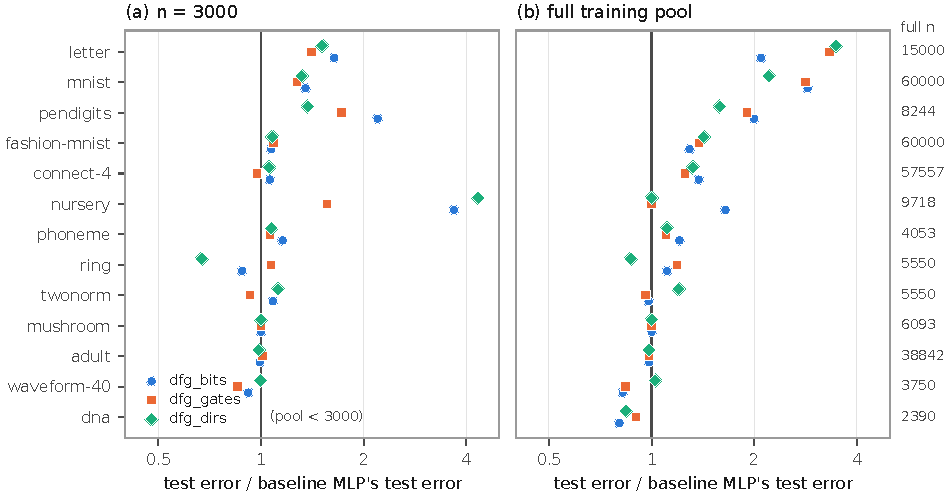
\includegraphics[width=\linewidth]{figures/fig_part7_ratio.pdf}
\caption{Part 7: test error of each DFG adaptation divided by the baseline MLP's, per held-out dataset, at $n=3000$ and at the full training pool (right column: its size). Errors are floored at 0.002, as in the study's $\log_2$ ratios. Datasets are sorted by the mean ratio at full $n$. Against the L2-regularized MLP, available for tabular data at $n\le3000$, the ratios in (a) are larger (\cref{tab:std}). On images at full $n$ the DFG adaptations are seed 0 only.}
\label{fig:part7}
\end{figure}

\Cref{tab:std} and \cref{fig:part7} give the results \status{Numerical}. The short answer is: not very well, beyond the toy problems.

\paragraph{Tabular data against the baseline MLP.} The error is on average 3--7\% higher (mean $\log_2$ ratio $+0.04$ to $+0.10$). Most cells are ties: DFG is better in 6--9 of 59 cells and worse in 10--15.

\paragraph{Tabular data against the L2-regularized MLP} ($n\le3000$). The error is 12--17\% higher ($+0.16$ to $+0.23$). The baseline MLP itself trails the regularized one by about the same amount ($+0.21$). So most of DFG's small-$n$ ``wins'' over the baseline were the baseline's lack of regularization. That was found by an independent audit, not anticipated. Of the 23 (learner, cell) wins over the baseline, 5 survive, all at $n\le300$:
\begin{itemize}
\item \code{dfg_bits} on dna at $n=300$: 0.060, against 0.119 for the regularized MLP and at least 0.10 for every MLP tried. It matches gradient boosting (0.057). Here sparse categorical motifs are exactly the bit-products DFG enumerates. Only this win also clearly beats every other reference.
\item \code{dfg_bits} on ring at $n=100$ and 300: 0.128 against 0.184, and 0.078 against 0.097.
\item \code{dfg_bits} and \code{dfg_gates} on waveform at $n=100$: 0.197 and 0.198, against 0.231.
\end{itemize}

\paragraph{Tabular data at full $n$.} DFG is clearly behind on tasks with many classes or interacting features:
\begin{itemize}
\item letter, 2.1--3.5$\times$ the MLP's error;
\item pendigits, 1.6--2.0$\times$;
\item connect\_4, 1.25--1.4$\times$.
\end{itemize}
Default gradient boosting has 8--12\% lower error than the three adaptations on held-out tabular data on average. It is lower on most datasets, but higher on twonorm and waveform.

\paragraph{Images.} DFG is behind from $n\approx3000$ on MNIST and from $n\approx10000$ on Fashion-MNIST, and roughly tied at small $n$. At $n=60000$:
\begin{itemize}
\item MNIST: 5.5--7.2\% error against the MLP's 2.5\% (2.2--2.9$\times$);
\item Fashion-MNIST: 14--16\% against 11\% (1.3--1.4$\times$).
\end{itemize}
All three adaptations are closer to logistic regression (7.8\% and 16.5\%) than to the MLP. \code{dfg_dirs}, whose dictionary is thresholded linear directions, the same kind of unit as an MLP's, is the best of the three on MNIST: 1.5$\times$ the MLP's error at $n=30000$ and 2.2$\times$ at 60000. The baseline MLP is somewhat under-tuned on images (2.5\% on MNIST at $n=60000$; Part 8's references reach 1.43--1.75\%, \cref{sec:images}). So the gap is probably a lower bound.

\paragraph{Compute.}
\begin{itemize}
\item \code{dfg_dirs} stayed within one MLP run in every cell by its own count (maximum 0.99).
\item \code{dfg_gates} exceeded it in 7 cells (maximum 1.07$\times$), because its final readout refit is not reserved in its budget check.
\item \code{dfg_bits} exceeded it on images, up to 3.45$\times$ on Fashion-MNIST at $n\ge10000$. It is behind the MLP in all those cells, and its lead over the other adaptations on Fashion-MNIST at $n\ge10000$ comes with 2--3.5$\times$ their compute.
\end{itemize}
An audit checked the FLOP counters against an instrumented count (\cref{app:compute}).

\subsection{Why it fails}\label{sec:whyfail}

DFG beat the networks on sparse Boolean targets because exhaustive search over a dictionary that contains the target's features pays only about $\ln N$ in samples (\cref{rem:lnN}), and the dictionary fit within the networks' FLOP budget. On standard tasks this premise fails in two ways \status{Heuristic}.

\paragraph{The useful features are continuous.} On images the useful hidden units are directions spread over hundreds of correlated pixels, each with a small weight. That is a continuous family.
\begin{itemize}
\item A product of a few bits, or a short AND of thresholds, is a poor approximation of such a direction.
\item DFG's directional moves (spectral directions, class discriminants, local mean differences) generate only a few candidate directions per round, from statistics of the current residual.
\item An MLP's gradient step updates hundreds of directions at once, each pulled toward the residual. In effect it is a continuous, parallel version of DFG's spectral move, iterated thousands of times.
\end{itemize}
In a continuous family, local search is the efficient search, and enumeration is not.

\paragraph{The tests can stall growth on dense signal.} Union-bound tests are built to stop false features on sparse targets. On dense real-world signal, many weak correlated effects, they stopped growth early on dev data; this is why \code{dfg_gates} lowered $c$. On held-out data, though, the largest losses (letter, pendigits, connect\_4, and images at large $n$) ran at or near the FLOP budget. There the dictionary and the budget, not the tests, are what bind. The MLP has no such gate. It moves all its units at once and controls overfitting with a continuous penalty, not by rejecting features. Here, L2 weight decay without early stopping lowered its error by 16\% at $n\le3000$.

\paragraph{What this does not show.}
\begin{itemize}
\item \emph{That no discrete learner can match MLPs.} Gradient boosting is also a discrete, greedily grown learner, and it beats the baseline MLP on several tabular datasets (adult, dna, ring). What does less well is DFG's specific recipe: exhaustive enumeration with union-bound tests over parity, gate or direction dictionaries. \Cref{sec:portfolio} follows this up.
\item \emph{That these adaptations are the best possible ones.} Each builder had about 70 minutes and only the dev data. \code{dfg_bits} and \code{dfg_gates} finished in about 20 minutes and \code{dfg_dirs} in about 50.
\item \emph{Anything about convolutional dictionaries.} None was tried on images.
\end{itemize}
